\chapter{مقدمه}
\label{chap:intro}

\begin{figure}
\includegraphics[width=\linewidth]{/ETCMobile/0GTo6G/mainFig}
\caption{\lofimage{/ETCMobile/0GTo6G/mainFig}
نسل‌های مختلف شبکه‌های تلفن‌همراه
}
\label{fig:0GTo6G}
\end{figure}
امروزه شاهد گسترش روزافزون شبکه‌های تلفن‌همراه در سرتاسر جهان هستیم. اطلاعات آماری حکایت از آن دارد که تا انتهای سال ۲۰۲۳ از میان 
$8.02$
میلیارد انسانی که بر روی کره زمین زندگی می‌کنند، در حدود 
$5.6$
میلیارد نفر از شبکه‌های تلفن‌همراه استفاده می‌کنند که این خود حاکی از
\gls{PenetrationCoefficient} $69$
درصدی این شبکه‌ها است. برطبق گزارش مؤسسه
\gls{GSMA}،
فناوری تلفن‌همراه و خدمات مرتبط با آن در سال 2023، در حدود 
$5.7$
تریلیون دلار ($5.4\%$ تولید ناخالص داخلی) ارزش‌افزوده به همراه داشته
\cite{GSMA2024MobileEconomy}.
این حجم شگرف چرخش مالی، منجر به ایجاد فرصت‌های پژوهشی، صنعتی و تجاری بسیاری گشته است. اهمیت شبکه‌های تلفن‌همراه، زمانی آشکار می‌گردد که بدانیم رشد و توسعه این شبکه‌ها، مرهون توسعه فناوری‌‌هایی نظیر 
\gls{MIMO}، \gls{IOT}، \gls{SDN}، \gls{NFV}و \gls{CloudComputing}
بوده است. این مهم به‌ویژه در شبکه‌های نسل پنج، بیش‌ازپیش خودنمایی می‌کند. 

شروع توسعه شبکه‌های نسل دو به‌مانند 
\gls{GSM}
در دهه 1980، با تمرکز بر ارائه خدماتی نظیر تبادل
\gls{Call} صوتی و \gls{SMS}
شکل گرفت. اما به‌مرور نقطه تمرکز به ارائه خدمات مبتنی بر 
\gls{PacketSwitch}
نیز معطوف گشت
(\gls{GPRS} و \lr{Edge}).
توسعه شبکه‌های نسل سه
\gls{UMTS}،
بسان پلی بود که ما را بیش‌ازپیش، بدین هدف نزدیک‌تر می‌نمود. در سال 2004، ایده‌های اولیه شبکه‌های نسل چهار 
(\gls{LTE} و \lr{LTE-Adv})،
با هدف ایجاد یک شبکه دسترسی با سرعت و ظرفیت بالا، قابلیت ارائه خدمات مختلف و انعطاف در تعامل با دیگر شبکه‌ها، تدوین گشت. در حال حاضر 
\lr{4G}
با سرعت سرسام‌آوری در حال توسعه جایگاه خویش در میان شبکه‌های تلفن همراه است، تا جایی که در سال 2018 در حدود 47 درصد کل ارتباطات تلفن همراه را به خود تخصیص داده است
\cite{globenewswire2019}. 




\gls{ITU} 
در پروژه‎ 
\lr{IMT-2020}، 
سه ویژگی کلیدی 
\lr{5G} 
را ارتباطات پرشمار ماشینی (مانند 
\lr{IoT})، 
پایدار و با 
\gls{Delay} 
اندک بر می‌شمارد. انتظار بر آن است که 
\lr{5G} 
از لحاظ پوشش، سرعت و تأخیر عملکرد چشمگیرتری نسبت به 
\lr{4G} 
از خود نشان دهد. برطبق نمودار 
\lr{Gartner} 
سرمایه‌گذاری و کار بر روی 
\lr{5G} 
حداقل تا یک دهه آینده ادامه خواهد داشت. تحقیقات بر روی شبکه‌های نسل جدید 
\lr{6G} 
از هم اکنون آغاز گشته و رد پای آن را در برخی از مقالات پژوهشی موجود در این حوزه می‌توان یافت 
(\autoref{fig:0GTo6G}).



\section{طرح مسئله}
هنگامی که کنوث پیش‌نمایش جلد دوم کتاب خود را
(\lr{The Art of Computer Programming})
در ۳۰ مارس ۱۹۷۷ دریافت کرد، متوجه شد که بسیار بدشکل است. در همین زمان بود که او کتاب
\lr{Artificial Intelligence}
نوشته
\lr{Patrick Winston}
که با حروف‌چینی دیجیتالی تهیه شده بود، را مشاهده نمود، و به این نوع از حروف‌چینی علاقه‌مند شد. پیش‌نمایش‌های مأیوس‌کننده در نهایت موجب شدند که او تصمیم بگیرد با طراحی سیستم حروف‌چینی خود برمبنای حروف‌چینی دیجیتالی، این مشکل را یک بار و برای همیشه حل کند. کنوث دریافت که معنای حروف‌چینی دیجیتالی این است که بتوان یک چیدمان درست از صفرها و یک‌ها (نقاط سفید و سیاه) را در کنار یکدیگر قرار داد. یافتن قواعد درست و زیبا برای نگارش متون ریاضی و تبدیل آن به چیدمان صحیحی از صفرها ویک‌ها، کاری بود که کنوث فکر می‌کرد آن‌را می‌تواند در ظرف شش ماه تا تعطيلات دانشگاهي سال ۱۹۷۸ به پایان برساند، اما آن‌چه که اتفاق افتاد این بود که در نهایت در ۱۹۸۹، یعنی ده سال بعد، این کار به اتمام رسید، و بدین‌سان 
\lr{\TeX{}}
متولد شد .... 

\lr{\TeX{}}
یک زبان نشانه‌گذاری
(\lr{Markup Language})
است.  محتوا در یک پروندهٔ متنی نوشته می‌شود و نشانه‌گذاری‌ها به شکل فرمان‌هایی بین متن قرارمی‌گیرند و مشخص می‌کنند که هر بخش از نوشته چه‌طور نمایش یابد. مفسر لاتک آن پرونده را می‌خواند، محتوا را به شکل یک نوشته درمی‌آورد و یک پروندهٔ خروجی می‌سازد. 
\begin{lstlisting}[language=TeX, numbers=none]
% Plain TeX for a 1 page document
\TeX{} is good at typesetting words like `fjord', `efficiency',
and `fiasco'. It is also good at typesetting math like,
$a^2 + b^2 = c^2$.
\beginsection 1. Introduction.
This is an example.
\bye
\end{lstlisting}
دقیقا برعکس نرم‌افزارهای واژه‌پرداز معمولی مثال 
\lr{Microsoft Word}
که بر اساس
\begin{center}
\lr{WYSIWYG (\textcolor{Plum}{\textit{What you see is what you get}})}
\end{center}
کار می‌کنند .... کنوث به کسانی که در 
\lr{\TeX{}}
 اشکالی بیابند و آن را گزارش کنند، جایزهٔ نقدی می‌دهد. جایزهٔ هر اشکال از 
$2.56$
 دلار آغاز شده و هر سال دو برابر شده‌است. این باعث فقر کنوث نشده‌است، چرا که تعداد بسیار کمی باگ گزارش شده‌است. علاوه بر این، افراد معمولاً به جای نقد کردن چک، آن را قاب می‌گیرند تا ثابت کنند در 
\lr{\TeX{}}
 اشکالی یافته‌اند.

\lr{\TeX{}}
یک زبان برنامه‌نویسی واقعی، گسترده و برای کاربر عادی بسیار مشکل است 
\lr{\LaTeX}
یک سامانه‌ی آماده‌سازی و حروف‌چینی نوشتار بر پایه
\lr{\TeX{}}
است، که از آن به عنوان موتور حروف‌چینی استفاده می‌کند.  در واقع هر دستور \lr{\LaTeX}، از مجموعه‌ای پیچیده از دستورات \lr{\TeX{}} تشکیل شده است، که گردابه‌ای بزرگ از صورت‌های توسعه‌یافته‌ی \lr{\TeX{}} را تشکیل می‌دهد. بدین‌سان خانواده 
\lr{\TeX{}}
روزبه‌روز گسترش یافت:
\lr{Xe\TeX{}}, \lr{Pdf\TeX{}}, \lr{Lua\TeX{}} و ... .

چرا باید از \LaTeX استفاده کنیم؟ به هزاران دلیل .....
\begin{itemize}
\tick \textcolor{Plum}{\textbf{جدابودن محتوا و ظاهر نوشته‌}}:
برتری بزرگ \lr{\LaTeX} در این موضوع برای کاربران \lr{Word} چندان واضح نیست، زیرا آن‌ها نمی‌دانند که این ویژگی چه‌قدر خوب است. وقتی با 
\lr{\LaTeX}
 نوشتهٔ خود را می‌نویسید، فقط به محتوای نوشته فکر می‌کنید و ساختار متن را مستقیماً به \lr{\LaTeX} می‌گویید ... 
\tick \textcolor{Plum}{\textbf{کیفیت}}:
به سختی می‌توان این موضوع را انکار کرد که کیفیت خروجی‌های لاتک بسیار فراتر از خروجی‌های
\lr{Word}
است.
\tick \textcolor{Plum}{\textbf{تسلط بر نوشته}}:
حتی در نوشته‌های کوتاه هم شاید شما با رفتار غیرهوشمندانهٔ \lr{Word} روبه‌رو شده‌باشید. مثلاً در یک نوشتهٔ ۳۰ صفحه‌ای پر از شکل و جدول، یک بعدازظهر را صرف می‌کنید تا همه‌چیز مرتب شود؛
\tick \textcolor{Plum}{\textbf{استانداردنویسی}}:
\lr{\LaTeX}
به شدت تلاش می‌کند تا شما را مجبور کند تا استاندارد بنویسید ... 
\tick \textcolor{Plum}{\textbf{رایگان}}:
در این مورد لاتک هیچ حرفی باقی نمی‌گذارد، چون رایگان است! ضرب‌المثل «هر چی بیشتر پول بدی، بیشتر آش می‌خوری» دربارهٔ لاتک صادق نیست.
\tick \textcolor{Plum}{\textbf{انعطاف‌پذیری}}:
می‌توانید با لاتک هرکاری که فکرش را می‌کنید انجام دهید! در طول سالیان دراز، بسته‌های بسیار زیادی ساخته شده‌اند که ویژگی‌های لاتک را گسترش می‌دهند. برای نمونه، بسته
\lr{Bibtex}, \lr{glossaries}, \lr{listings}, \lr{tikz} و .... .
\tick \textcolor{Plum}{\textbf{پایداری‌}}: \lr{Word} 
در هنگام ویرایش نوشته‌های طولانی زیاد قفل می‌کند، اما 
\lr{\TeX{}} .... . 
\tick \textcolor{Plum}{\textbf{امنیت‌}}:
 در لاتک نیازی نیست نگران ویروس‌هایی باشید که در ماکروهای \lr{Word} پنهان می‌شوند!
\tick \textcolor{Plum}{\textbf{مستقل از سیستم‌عامل}}
\tick \textcolor{Plum}{\textbf{انجمن‌های پرسش و پاسخ بسیار قوی}}
\end{itemize}

برای من این تغییر کاملاً سودآور بود، زیرا الان می‌توانم نوشته‌ها و گزارش‌هایم را با سرعت بیشتری بنویسم. هرکسی می‌تواند لاتک را امتحان کند و تفاوتش را ببیند و تصمیم بگیرد. اما هر کس که وارد دنیای
\lr{\LaTeX}
در آن غرق شد ... 

\begin{figure}
\includegraphics[width=0.9\linewidth]{/calcdistance/mainFig}
\caption{\lofimage{/calcdistance/mainFig}%
نمونه شکل ساخته شده با 
\lr{Tikz}}
\label{fig:cellgeom}
\end{figure}

\section{چالش‌ها و انگیزه}

\section{نوآوری‌ها}
نوآوری‌های این پایان‌نامه به طور خلاصه به شرح زیر است:
 \begin{itemize} 
 \tick 
ارایه یک روش نوین برای بهینه‌سازی ....
 \end{itemize}
 

\section{ساختار گزارش}
نخست در
\autoref{chap:concepts}،
تعاریف و مفاهیم مبنایی در حوزه‌ی شبکه‌های تلفن همراه مانند معماری 
\gls{UE}
بیان می‌شود. در
\autoref{chap:relatedworks}،
به معرفی و بررسی کارهای پیشین انجام شده در این حوزه پرداخته خواهد شد. در 
\autoref{chap:approach}،
روش پیشنهادی این پژوهش ارائه خواهد شد که شامل استفاده از داده‌های جمع‌آوری‌شده از \gls{DriveTest}، مدل‌سازی کانال، و به‌کارگیری روش‌های هوش مصنوعی برای پیش‌بینی دقیق‌تر و بهبود عملکرد شبکه است. در 
\autoref{chap:simulation}
نتایج به‌دست‌آمده از آزمایش‌های متعدد روش پیشنهادی را تحلیل کرده و در نهایت در
\autoref{chap:conclusion}
به جمع‌بندی این پژوهش خواهیم پرداخت.
